\refstepcounter{chapter}
\addcontentsline{toc}{chapter}{General Description of the Machine}

\setsectiontitle{Technical Data}
\setrevision{5628}

\subsection{Work Area}
Adjustment of the cross support:
\begin{itemize}
    \item in the horizontal longitudinal axis (X-axis): \dotfill 400 mm
    \item in the vertical axis (Y-axis): \dotfill 375 mm
\end{itemize}

Adjustment of the spindle head:
\begin{itemize}
    \item in the horizontal transverse axis (Z-axis): \dotfill 250 mm
\end{itemize}

\subsection{Workspace}
Vertical mounting table \footnotemark[4]
\begin{itemize}
    \item Clamping surface: \dotfill 510 x 800 mm
    \item Number of guide grooves: \dotfill 1
\end{itemize}

\footnotetext[4]{Worktables, see Section 4 of the technical documentation.}

\subsection{Working Spindles}
\begin{itemize}
    \item Tool holder:\footnotemark[5] \dotfill ISO 40
    \item Quill stroke of the vertical working spindle: \dotfill 50 mm
    \item Clamping force of the tool clamp ISO-Type B Clamping pin: \dotfill N \footnotemark[6]
    \item MAHO-OTT Clamping groove: \dotfill N \footnotemark[6]
\end{itemize}

\footnotetext[5]{For tool holding according to DIN 69871, with pull studs ISO 7388, Type B.}
\footnotetext[6]{Tool clamping, see sheet 3.12-1; tool holders, see sheets 3.13-1 and 3.13-3.}

\subsection{Speeds and Feeds}
Working spindle speeds,\footnotemark[7] \\Directly programmable: \dotfill 80 - 4000 rpm

\footnotetext[7]{Transmission with 18 speed levels and a manual shifting step of 1.25, controlled by CNC and manually switchable.}

Feeds, directly programmable: \footnotemark[8]
\begin{itemize}
    \item In the X, Y, Z axes: \dotfill 0.1 - 1500 mm/min
\end{itemize}

\footnotetext[8]{Minimum feed rate in axes X, Y, Z: 1 mm/min.}

Rapid traverse:
\begin{itemize}
    \item In the X, Y, Z axes: \dotfill 2.5 m/min
\end{itemize}

\newpage
\subsection{Electrical Equipment}
\begin{itemize}
    \item Voltage: \dotfill 220/380 V \footnotemark[9]
    \item Frequency: \dotfill 50/60 Hz \footnotemark[9]
    \item Total connected load of the machine: \dotfill 11 kVA \footnotemark[9]
\end{itemize}

\footnotetext[9]{Standard configuration.}

\subsection{CNC Control\textsuperscript{\ref{fn:control}}}
\begin{itemize}
    \item Resolution of the linear measurement systems: \dotfill 0.001 mm
    \item Display of measured values: \dotfill Screen
    \item Number of simultaneously controlled axes: \dotfill 2
    \item Number of sequentially controlled axes: \dotfill 3
\end{itemize}

\footnotetext[10]{The CNC control is described in a separate manual.\label{fn:control}}

\subsection{Weight and Space Requirements}
Weight of the machine (with vertical milling head, \\
fixed table, and control cabinet), approx.:\dotfill 1,250 kg

Space requirements (without expansion dimensions):
\begin{itemize}
    \item Length: \dotfill 2,310 mm
    \item Width: \dotfill 2,475 mm
    \item Height: \dotfill 1,830 mm
\end{itemize}

\setsectiontitle{Machine Overview}
\setrevision{7631}

\subsection*{Main Components Overview} % Unnumbered subsection for the first page title

\begin{figure}[h]
    \centering
    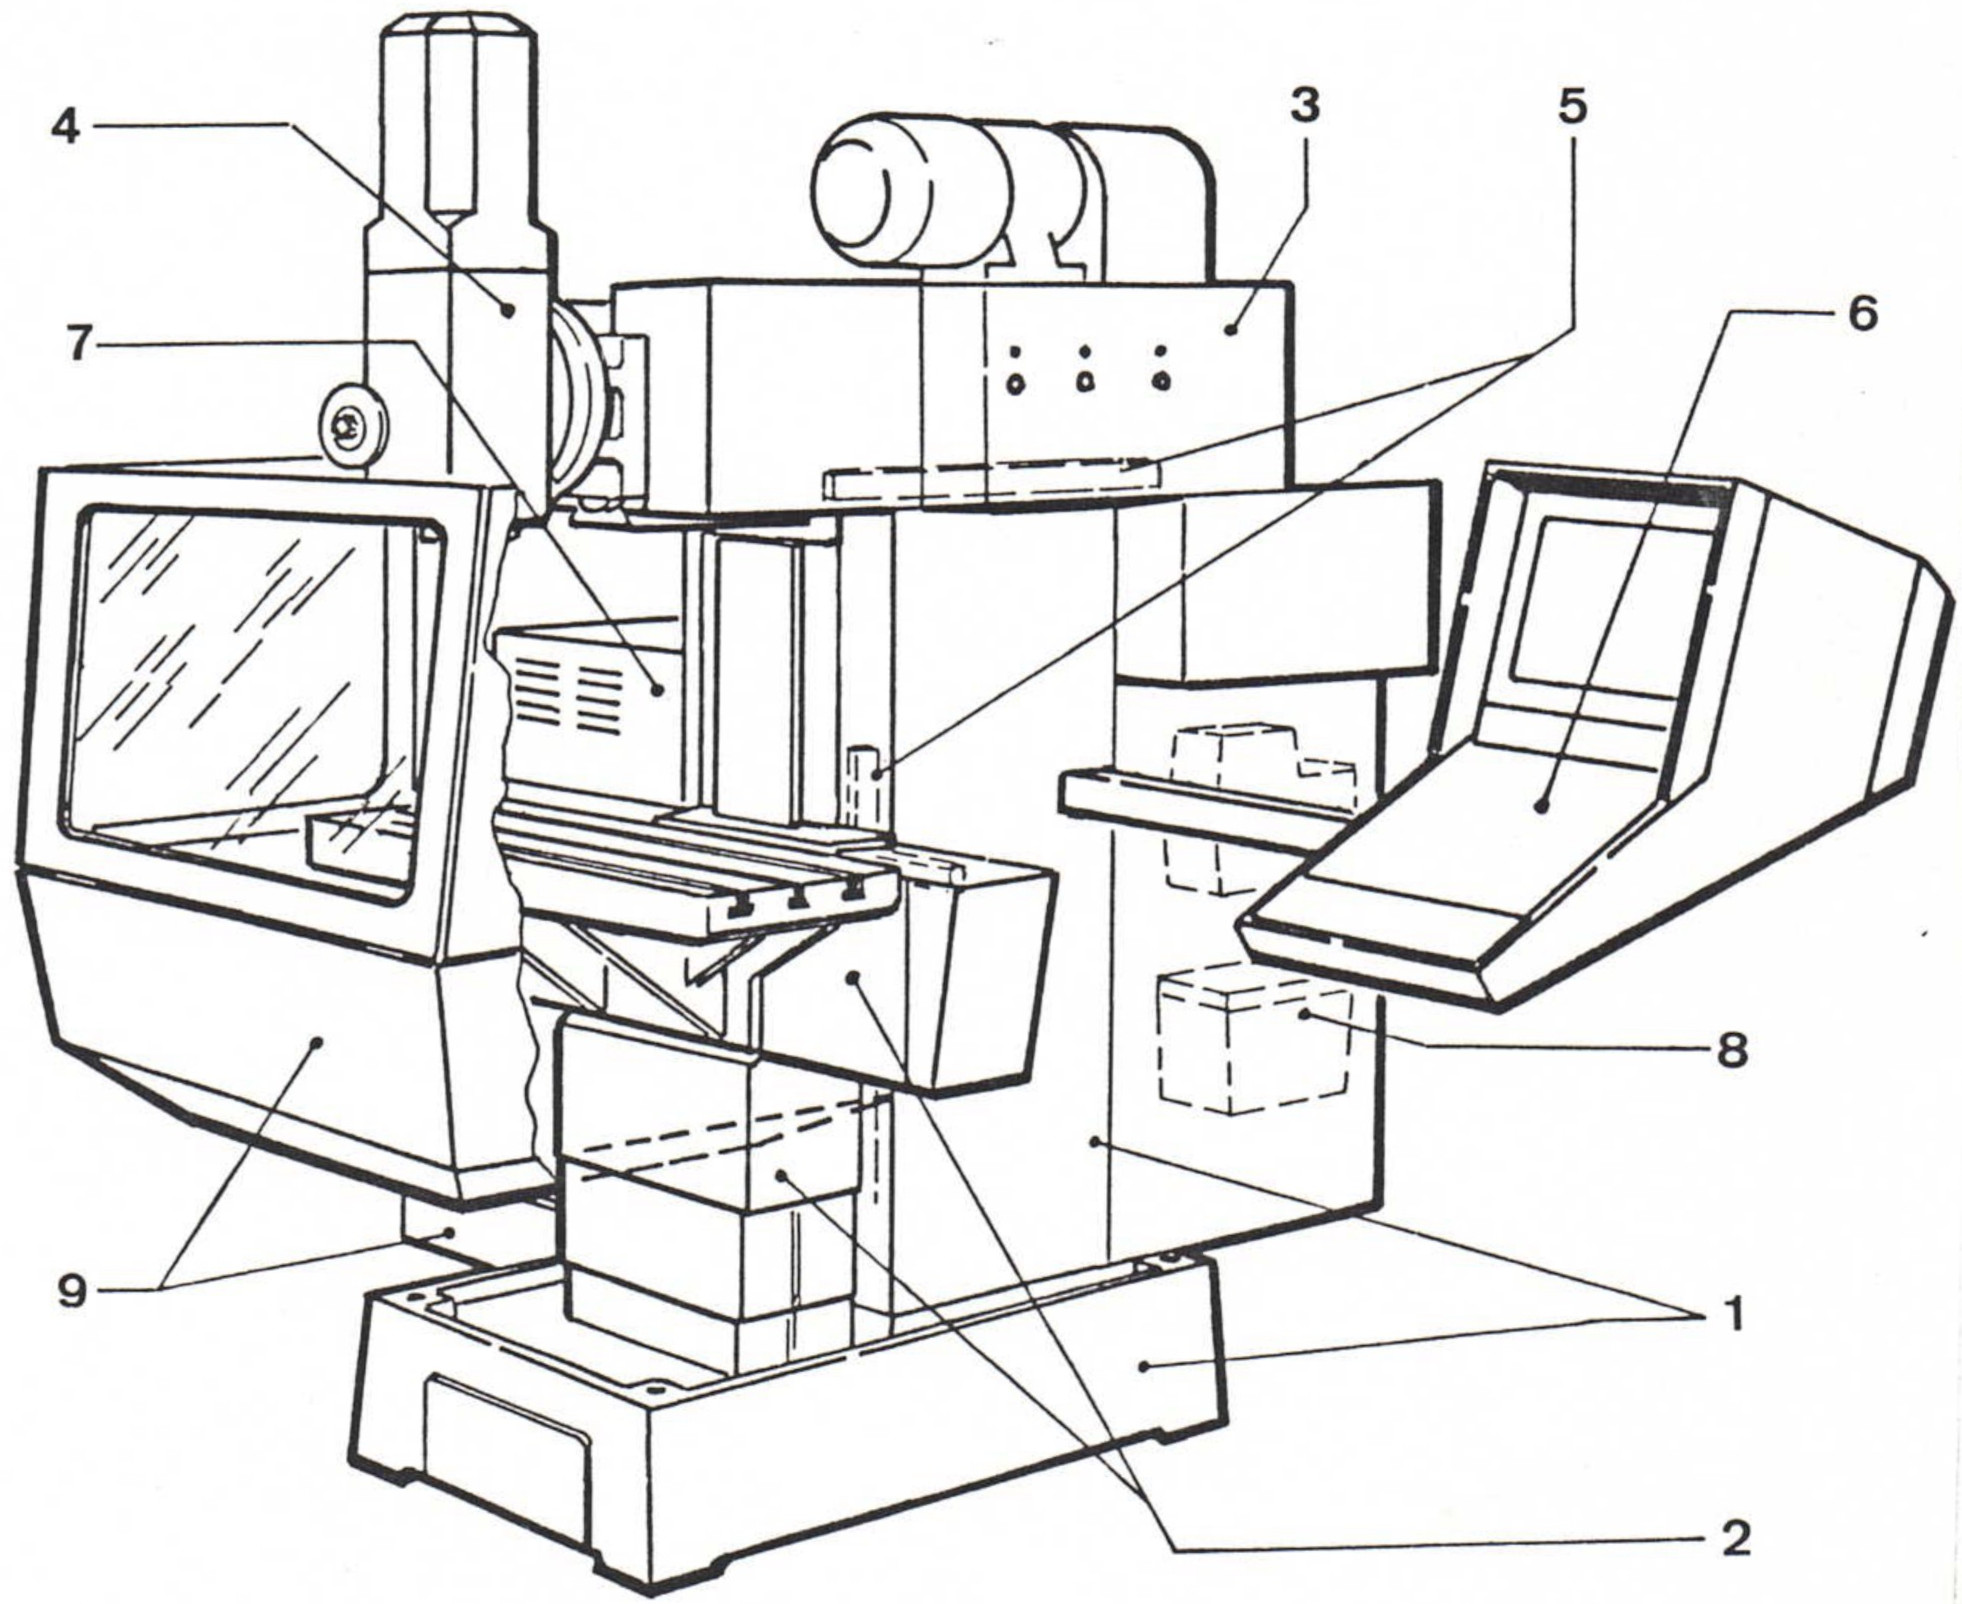
\includegraphics[width=0.8\textwidth]{chapter2/machine_overview.jpg}
    \caption{}
    \label{fig:machine_overview}
\end{figure}

\vspace{3cm}

\begin{enumerate}[itemsep=1pt,parsep=0pt]
    \item Machine stand with base and Y-axis feed drive
    \item Cross support with vertical mounting table and X-axis feed drive
    \item Spindle head with horizontal working spindle and Z-axis feed drive
    \item Vertical milling head with vertical working spindle
    \item Measuring systems
    \item CNC control
    \item Electrical system
    \item Central lubrication system / hydraulic system
    \item Coolant system / splash guard
\end{enumerate}

\notebox{NOTE}{Description of the operating elements for the worktables can be found in Section 4 of the operator's manual.}

\subsection{Machine Stand with Base}

\begin{figure}[h]
    \centering
    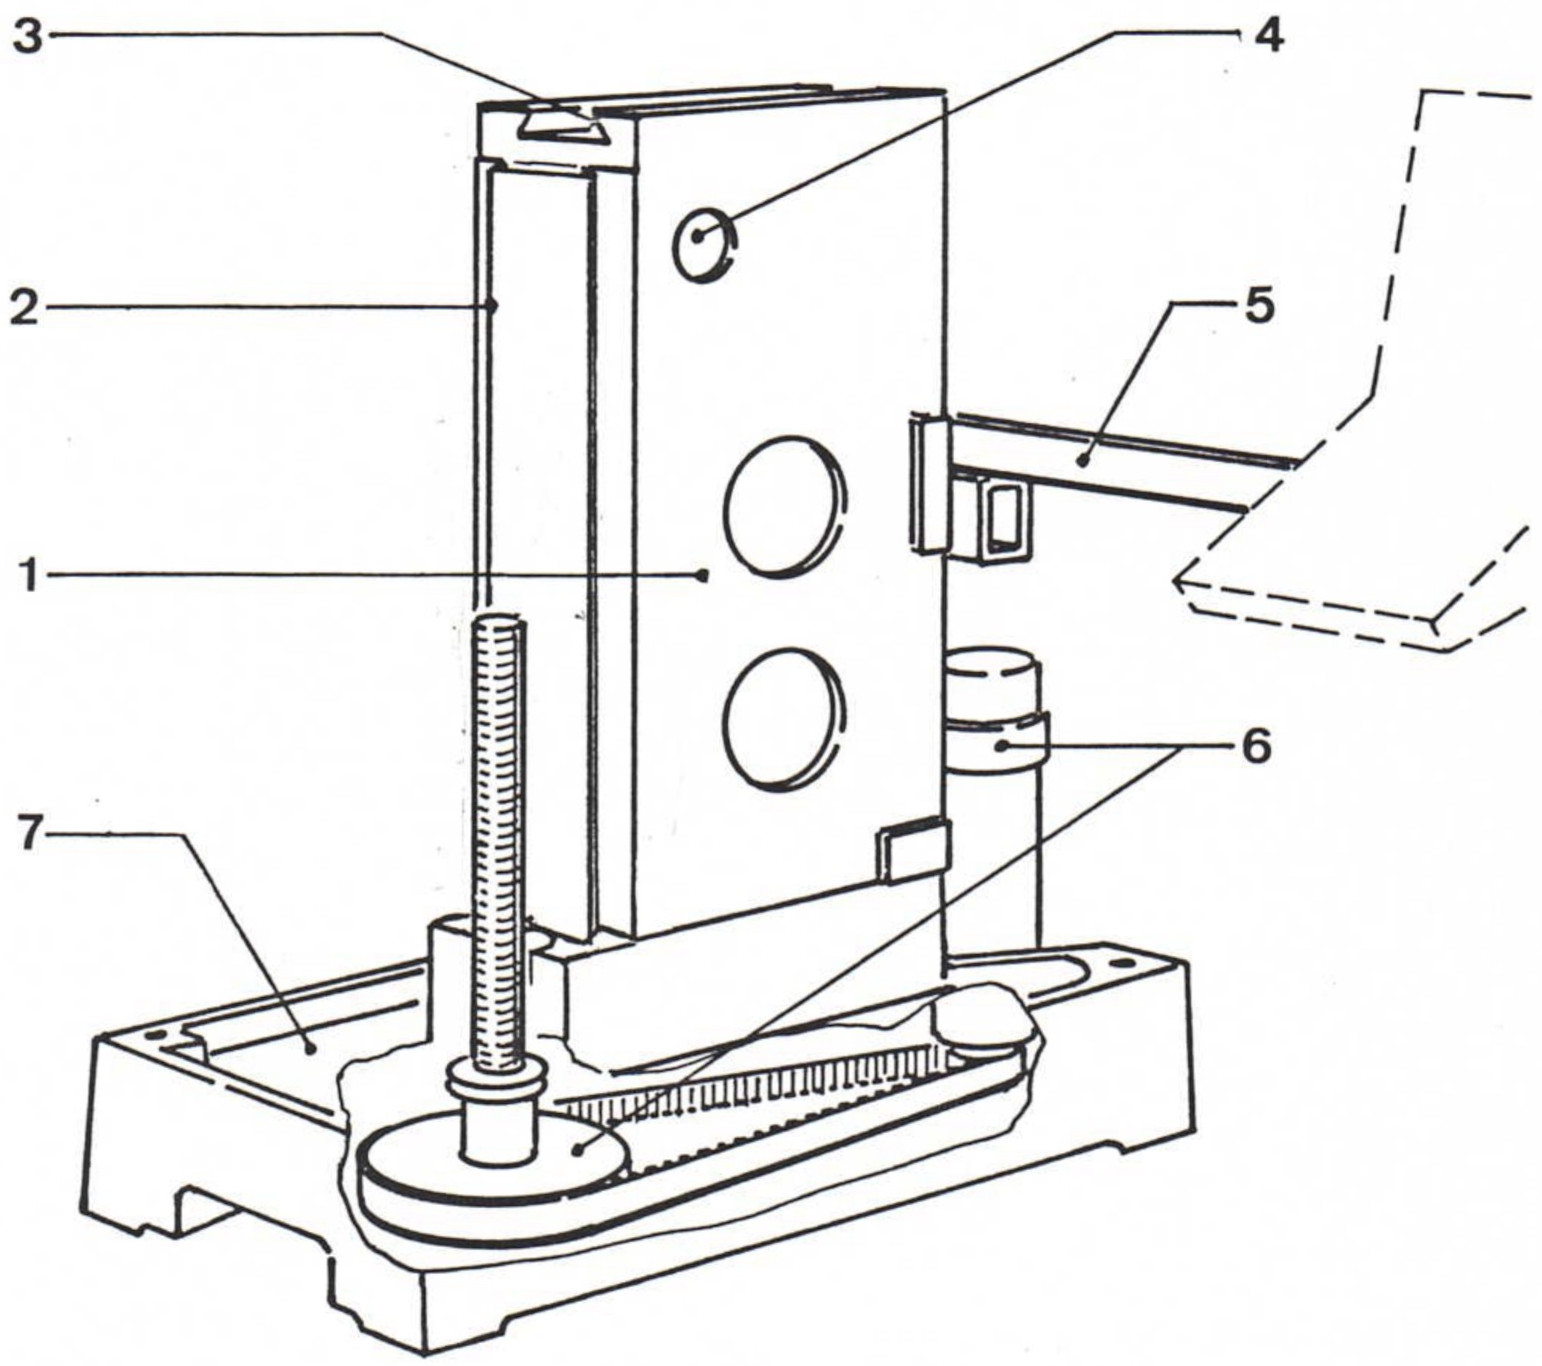
\includegraphics[width=0.6\textwidth]{chapter2/machine_stand.jpg}
    \caption{Diagram of the machine stand and its components.}
    \label{fig:machine_stand}
\end{figure}

The numbered components in the diagram are:
\begin{enumerate}[itemsep=1pt,parsep=0pt]
    \item Machine stand
    \item Dovetail guide for cross support
    \item Spindle head guide
    \item Opening for transporting the machine
    \item Swivel arm for control panel
    \item Y-axis feed drive
    \item Stand base
\end{enumerate}

The machine stand (1) with stand base (7) serves as the structural support for the other assemblies.

The dovetail guide (2) on the front allows the vertical slide of the cross support to move smoothly.

The mating surfaces of the spindle head (3) on the upper section of the \\machine stand are coated with the same plastic sliding material as the mating surface of the cross support.

In the upper half of the stand, there is a continuous opening (4) designed to accommodate the transport rod.

The Y-axis feed drive (6) is housed within the stand base (7).

\vfill
\clearpage

\subsection{Cross Support}

\begin{minipage}{0.5\textwidth}
    \begin{enumerate}[itemsep=1pt,parsep=0pt]
        \item Longitudinal slide
        \item Vertical slide, Y-axis
        \item DC motor, Y-axis
        \item Timing belt, Y-axis
        \item Ball screw, Y-axis
        \item Dovetail guide, Y-axis
        \item Ball screw, X-axis
        \item Timing belt, X-axis
        \item DC motor, X-axis
        \item Dovetail flat guide, X-axis
    \end{enumerate}
\end{minipage}%
\begin{minipage}{0.5\textwidth}
    \centering
    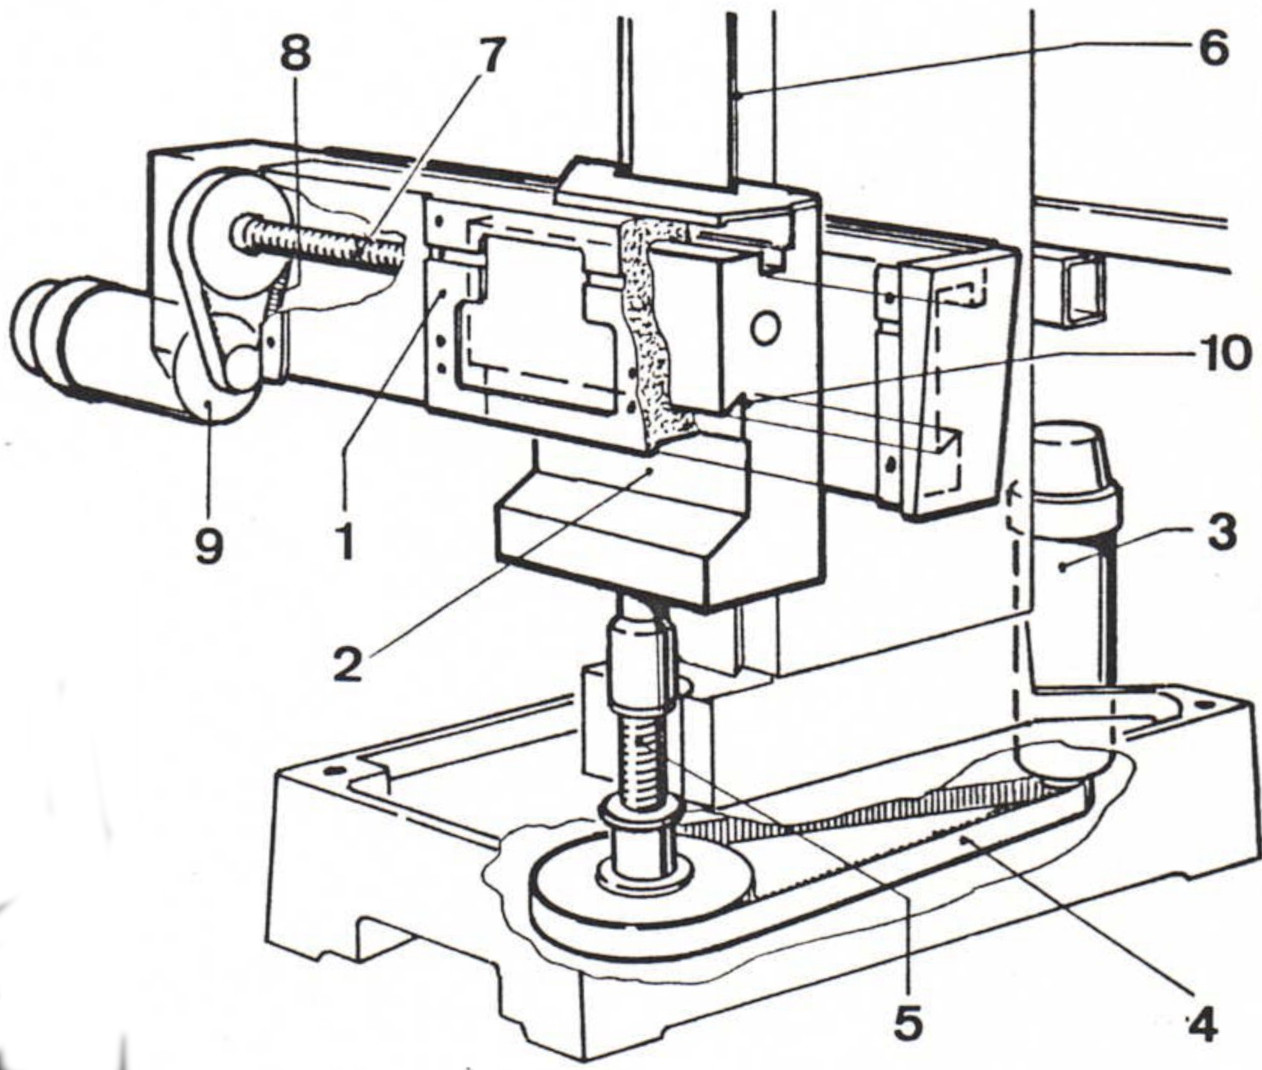
\includegraphics[width=0.9\textwidth]{chapter2/cross_support.jpg}
    \captionof{figure}{}
    \label{fig:cross_support}
\end{minipage}

\vspace{1cm}

The cross support carries out the necessary longitudinal and vertical\\ movements for workpiece machining.

It consists of the longitudinal slide "vertical mounting table" (X-axis) (1) and the vertical slide (Y-axis) (2).

The worktables are mounted on the vertical mounting table; see Chapter 4.

A DC motor (3), along with timing belts (4) and a ball screw (5), provides the feed drive for the Y-axis.

The vertical slide moves along the dovetail guide (10) on the machine stand. The mating surfaces on the support are coated with a plastic sliding material that has excellent wear resistance, emergency running properties, damping characteristics, and friction performance, allowing smooth sliding \\(eliminating the stick-slip effect).

The longitudinal slide is guided by the vertical slide using a dovetail guide (6). Its mating surfaces are also coated with the specialized sliding \\material.

All guides are equipped with wipers to protect against chips, dirt, and \\coolant contamination and are automatically lubricated via a central \\lubrication system.

The longitudinal slide (X-axis) is driven by a DC motor (9) through a timing belt (8) and a ball screw (7).

\vfill
\clearpage

\subsection{Spindle Head}

\begin{minipage}{0.5\textwidth}
    \begin{enumerate}[itemsep=1pt,parsep=0pt]
        \item Spindle head housing
        \item Main motor
        \item Gearbox
        \item Poly V-belt
        \item Timing belt
        \item DC motor, Z-axis
        \item Ball screw
        \item Horizontal working spindle
        \item Vertical milling head drive shaft
    \end{enumerate}
\end{minipage}%
\begin{minipage}{0.5\textwidth}
    \centering
    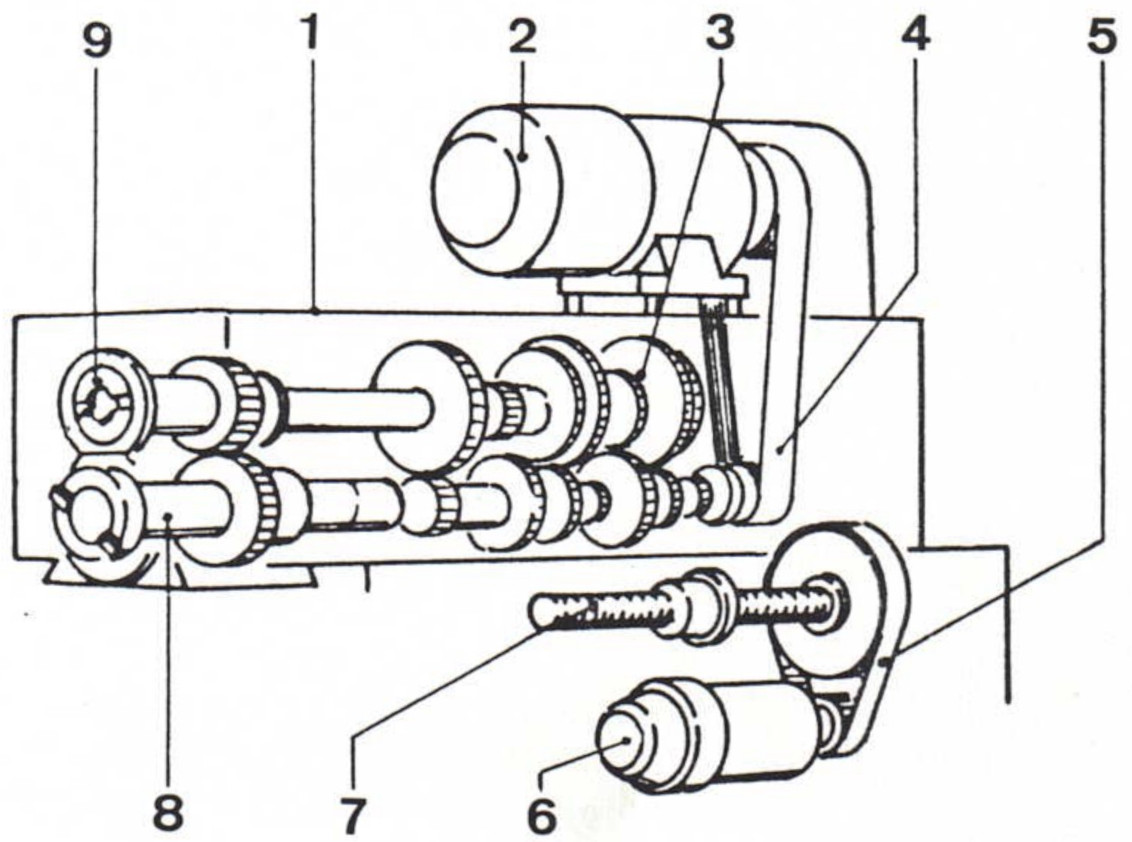
\includegraphics[width=0.9\textwidth]{chapter2/spindle_head.jpg}
    \captionof{figure}{}
    \label{fig:spindle_head}
\end{minipage}

\vspace{1cm}

The spindle head (1) is equipped with a dovetail guide and is mounted on the upper side of the machine stand.

Its front side accommodates either the vertical milling head or the \\counterholder for horizontal milling (see also pages 3.05-1, 3.07-1 to \\3.09-1).

The dovetail guide is fitted with wipers to prevent the ingress of chips, dirt, and coolant.

The mating surfaces on the machine stand are coated with the same specialized sliding material as those on the cross support.

The three-phase main motor (2) is mounted on top of the spindle head.

The main motor's torque is transmitted via a poly V-belt (4) and an integrated 18-speed gearbox (3) within the spindle head to the working spindle (8).

The working spindle (8) runs in five preloaded precision spindle bearings, which are permanently lubricated for maintenance-free operation.

A DC motor (6) mounted beneath the spindle head, together with the timing belt (5) and ball screw (7), drives the Z-axis feed motion.

\vfill
\clearpage

\subsection{Vertical Milling Head}

\begin{minipage}{0.5\textwidth}
    \begin{enumerate}[itemsep=1pt,parsep=0pt]
        \item Spindle head
        \item Milling head extension arm
        \item Intermediate flange
        \item Milling head housing
        \item Vertical working spindle
        \item Quill adjustment mechanism
    \end{enumerate}
\end{minipage}%
\begin{minipage}{0.5\textwidth}
    \centering
    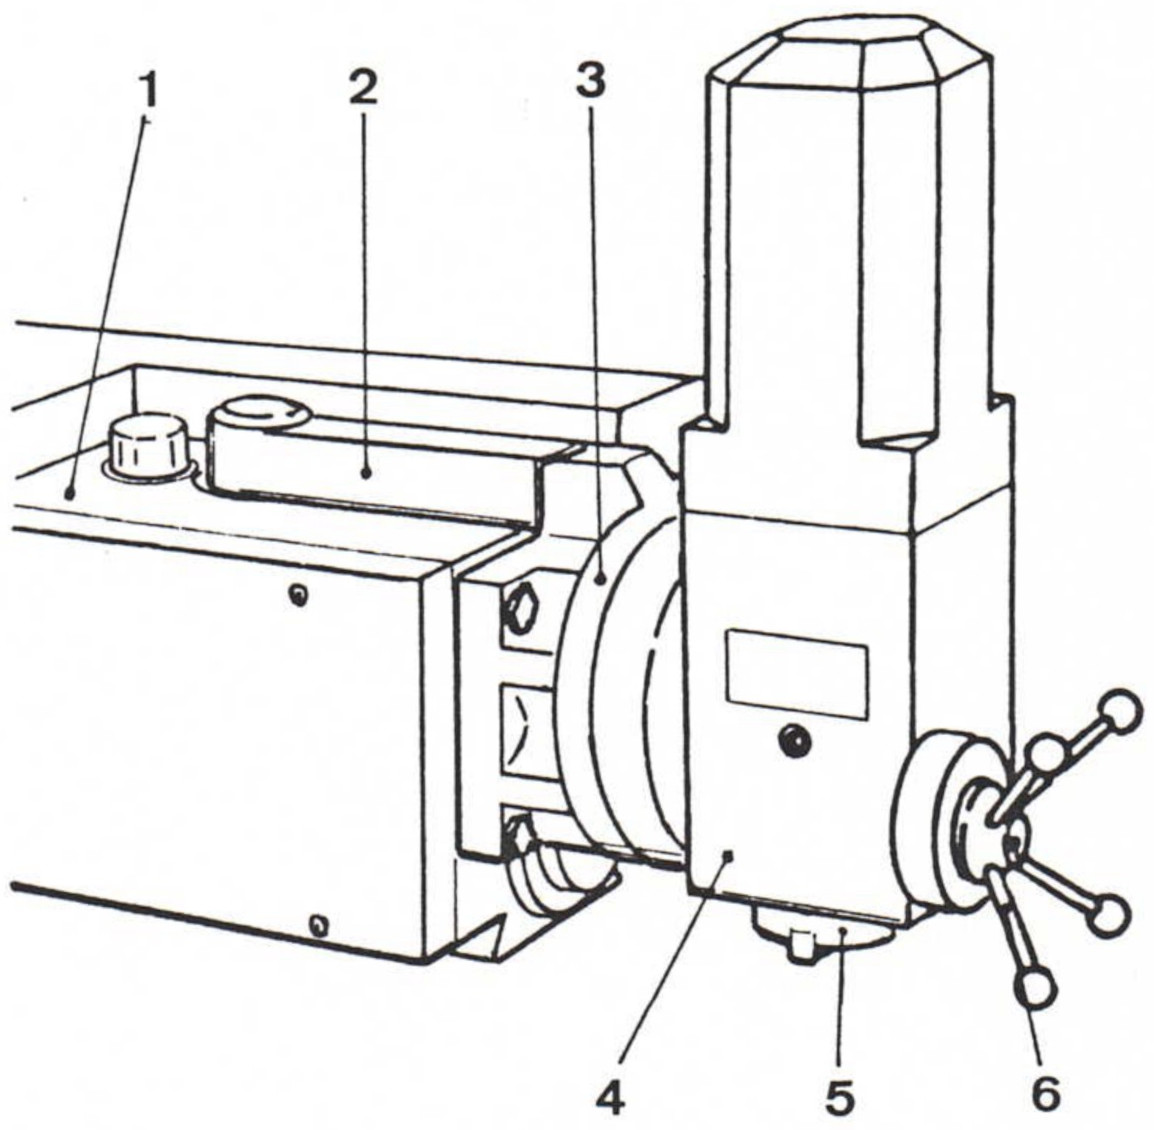
\includegraphics[width=0.9\textwidth]{chapter2/vertical_milling_head.jpg}
    \captionof{figure}{}
    \label{fig:vertical_milling_head}
\end{minipage}

\vspace{1cm}

The vertical milling head is mounted on top of the spindle head (1) with a pivotable extension arm. This allows it to be swung out of the working area when not in use.

The milling head housing (4) is mounted on the intermediate flange (3) and can be swiveled 90° in both directions.

The vertical working spindle (5) is supported by four preloaded precision spindle bearings within a quill. Due to its lifetime lubrication, these bearings are maintenance-free.

The quill can be extended using the quill adjustment mechanism (6).

Detailed instructions on operation and handling can be found on pages 3.07-1 to 3.09-1.

\newpage
\subsection{Measuring Systems}

The measuring systems operate contact-free and maintenance-free, with a \\resolution of 0.001 mm. Protective covers shield them from the ingress of chips and coolant.

A detailed functional description of the measuring systems can be found in Chapter 5.

The X-axis measuring system is installed at the top of the cross support.

The Y-axis measuring system is located on the left side of the machine stand.

The Z-axis measuring system is mounted on the left side of the spindle head.

Thermal expansion of the spindle head, caused by the working spindle heating up, is compensated by the Z-axis measuring system.

To ensure high measurement accuracy, an invar rod (2) fixed to the spindle head compensates for thermal expansion by adjusting the scale bar (4), \\maintaining precise measurements throughout the machine's operational life.

\vspace{0.5cm}

\textbf{\uline{Z-Axis Measuring System}}

\begin{figure}[h]
    \centering
    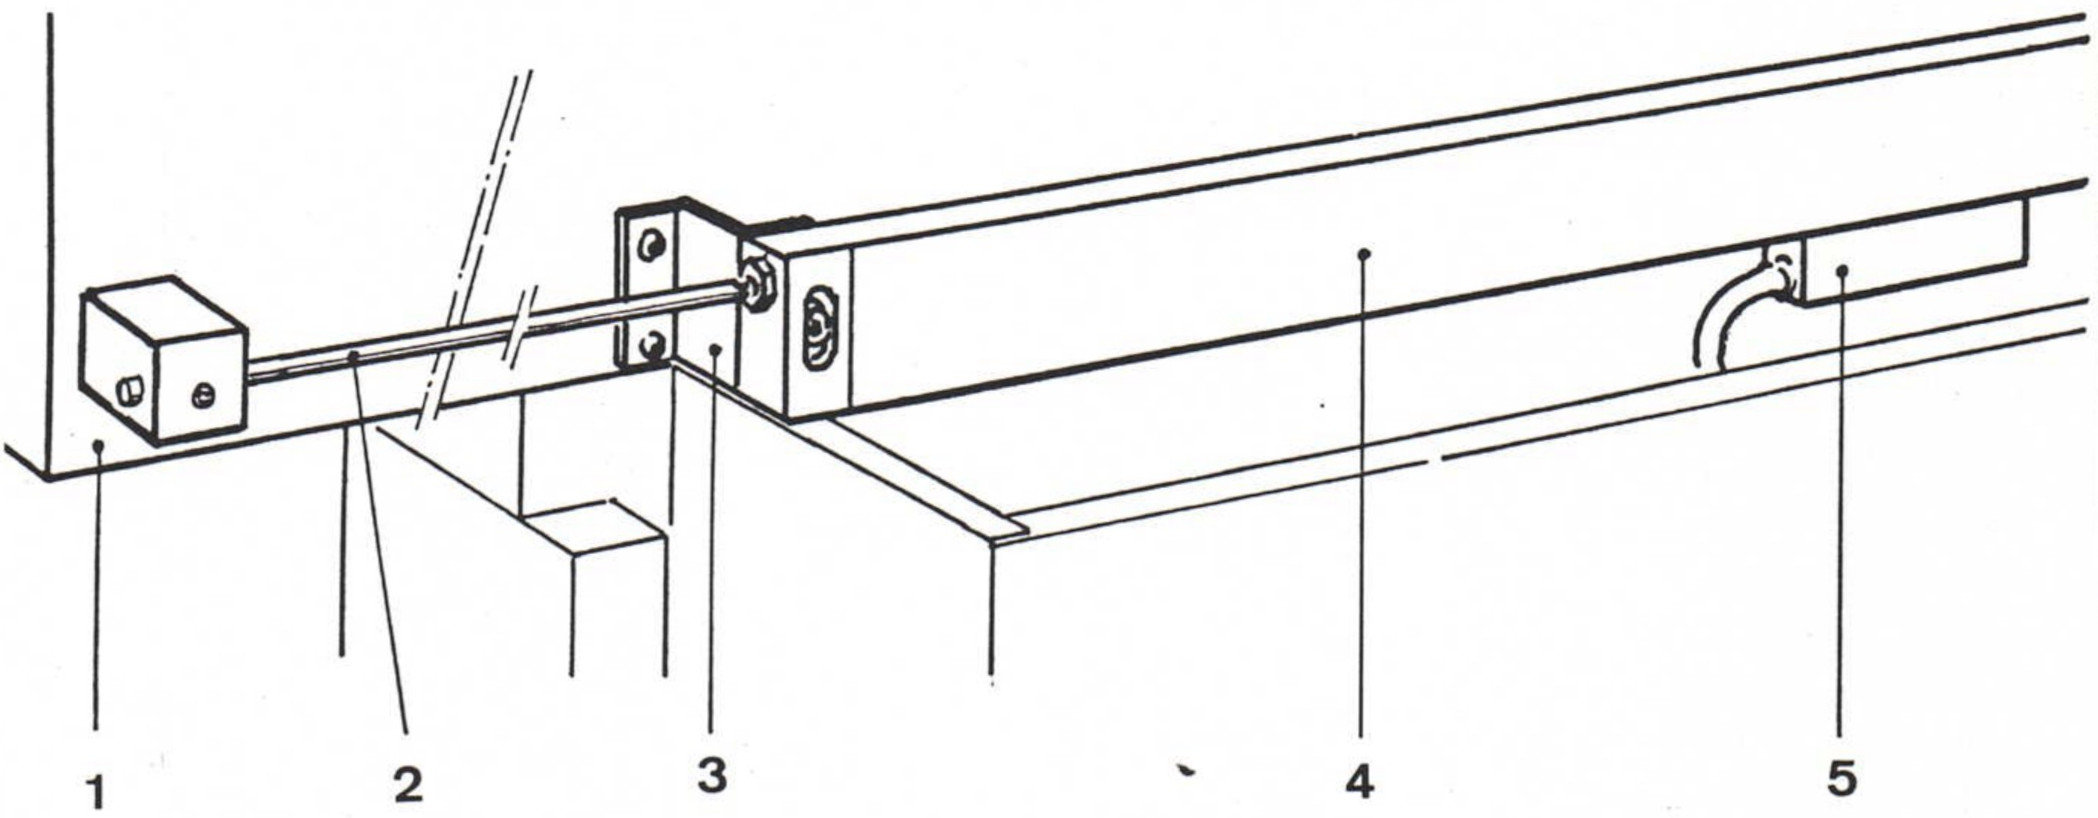
\includegraphics[width=0.9\textwidth]{chapter2/measuring_system_z_axis.jpg}
    \caption{}
    \label{fig:measuring_system_z}
\end{figure}

\begin{enumerate}[itemsep=1pt,parsep=0pt]
    \item Spindle head
    \item Invar rod
    \item Suspension strips
    \item Scale bar, Z-axis
    \item Measuring head
\end{enumerate}

\newpage

\subsection{CNC Control 432 E/Graphics}

The CNC control unit is housed in the control cabinet (5), while the control panel (2) and screen (3) are mounted in a control console. This console (4) is rotatable and is attached to a swivel arm (1) on the left side of the machine.

The construction, function, and programming of the control system are \\described in the CNC 432/10-Graphics manual.

\vspace{-.3cm}


\begin{minipage}[b]{0.5\textwidth}
    \textbf{\uline{CNC Control 432 E/Graphics}}
    \begin{enumerate}[itemsep=1pt,parsep=0pt]
        \item Swivel arm
        \item Control panel
        \item Screen
        \item Control console
    \end{enumerate}
\end{minipage}%
\begin{minipage}{0.5\textwidth}
    \centering
    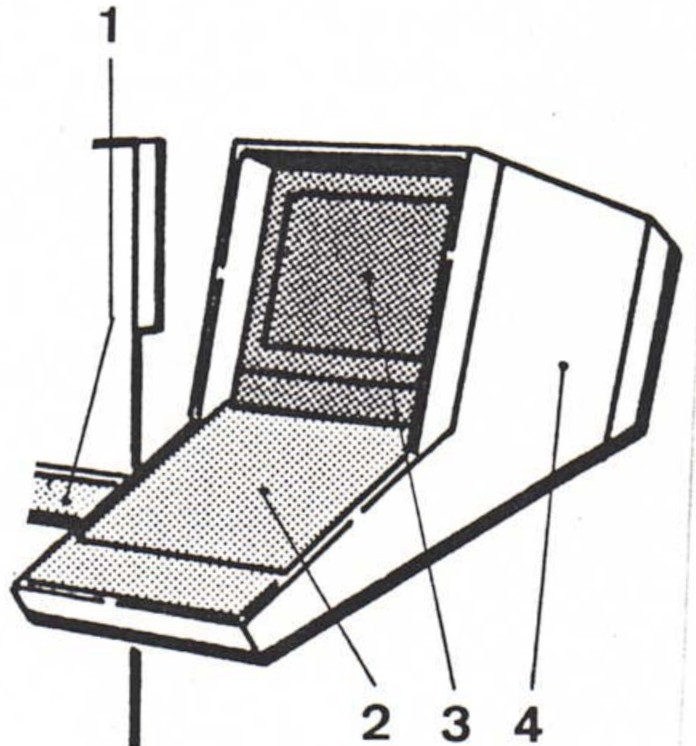
\includegraphics[width=0.6\textwidth]{chapter2/cnc_control.jpg}
    \captionof{figure}{}
    \label{fig:cnc_control}
\end{minipage}

\vspace{-1cm}

\subsection{Electrical System}

The control cabinet (5), located at the rear of the machine, contains the power module, which supplies energy to the machine’s drives.

It processes signals from the CNC 432 E control, regulates the drives, and protects against overcurrent.

Inside the control cabinet door (8) are the main switch (9) and the adjustment module (10).

\begin{minipage}[c]{0.45\textwidth}
    \begin{enumerate}[itemsep=1pt,parsep=0pt]
        \setcounter{enumi}{4}
        \item Control cabinet
        \item Transformer room
        \item Heat exchanger
        \item Control cabinet door
        \item Main switch
        \item Adjustment module
        \item CNC Control 432 E/Graphics
    \end{enumerate}

    The adjustment module contains the following switches:
\end{minipage}%
\begin{minipage}{0.6\textwidth}
    \centering
    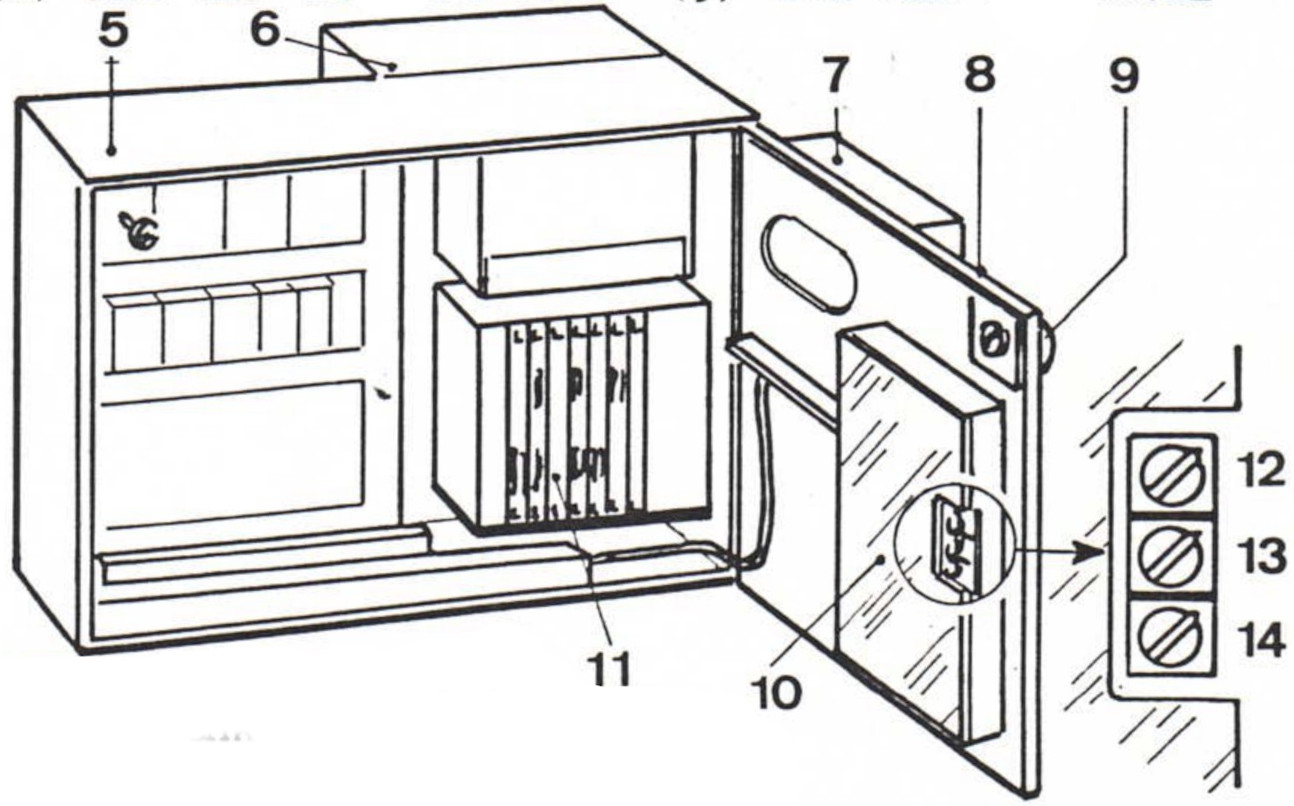
\includegraphics[width=\textwidth]{chapter2/electrical_system.jpg}
    % \captionof{figure}{}
    \label{fig:electrical_system}
\end{minipage}

\begin{textblock*}{\textwidth}(3cm, 21cm)  % Adjust coordinates as needed
    \begin{enumerate}[itemsep=1pt,parsep=0pt]
        \setcounter{enumi}{11}
        \item \textbf{Rotary switch (7S1):} "Brake Y-axis engaged/disengaged"
        \item \textbf{Rotary switch (19S1):} "Read machine constants"
        \item \textbf{Rotary switch (19S2):} "Test operation"
    \end{enumerate}
\end{textblock*}

\vspace{2cm}

\notebox{NOTE}{The numbers in parentheses correspond to circuit diagram labels.}

\setsectiontitle{Movement Directions}

\begin{figure}[h]
    \centering
    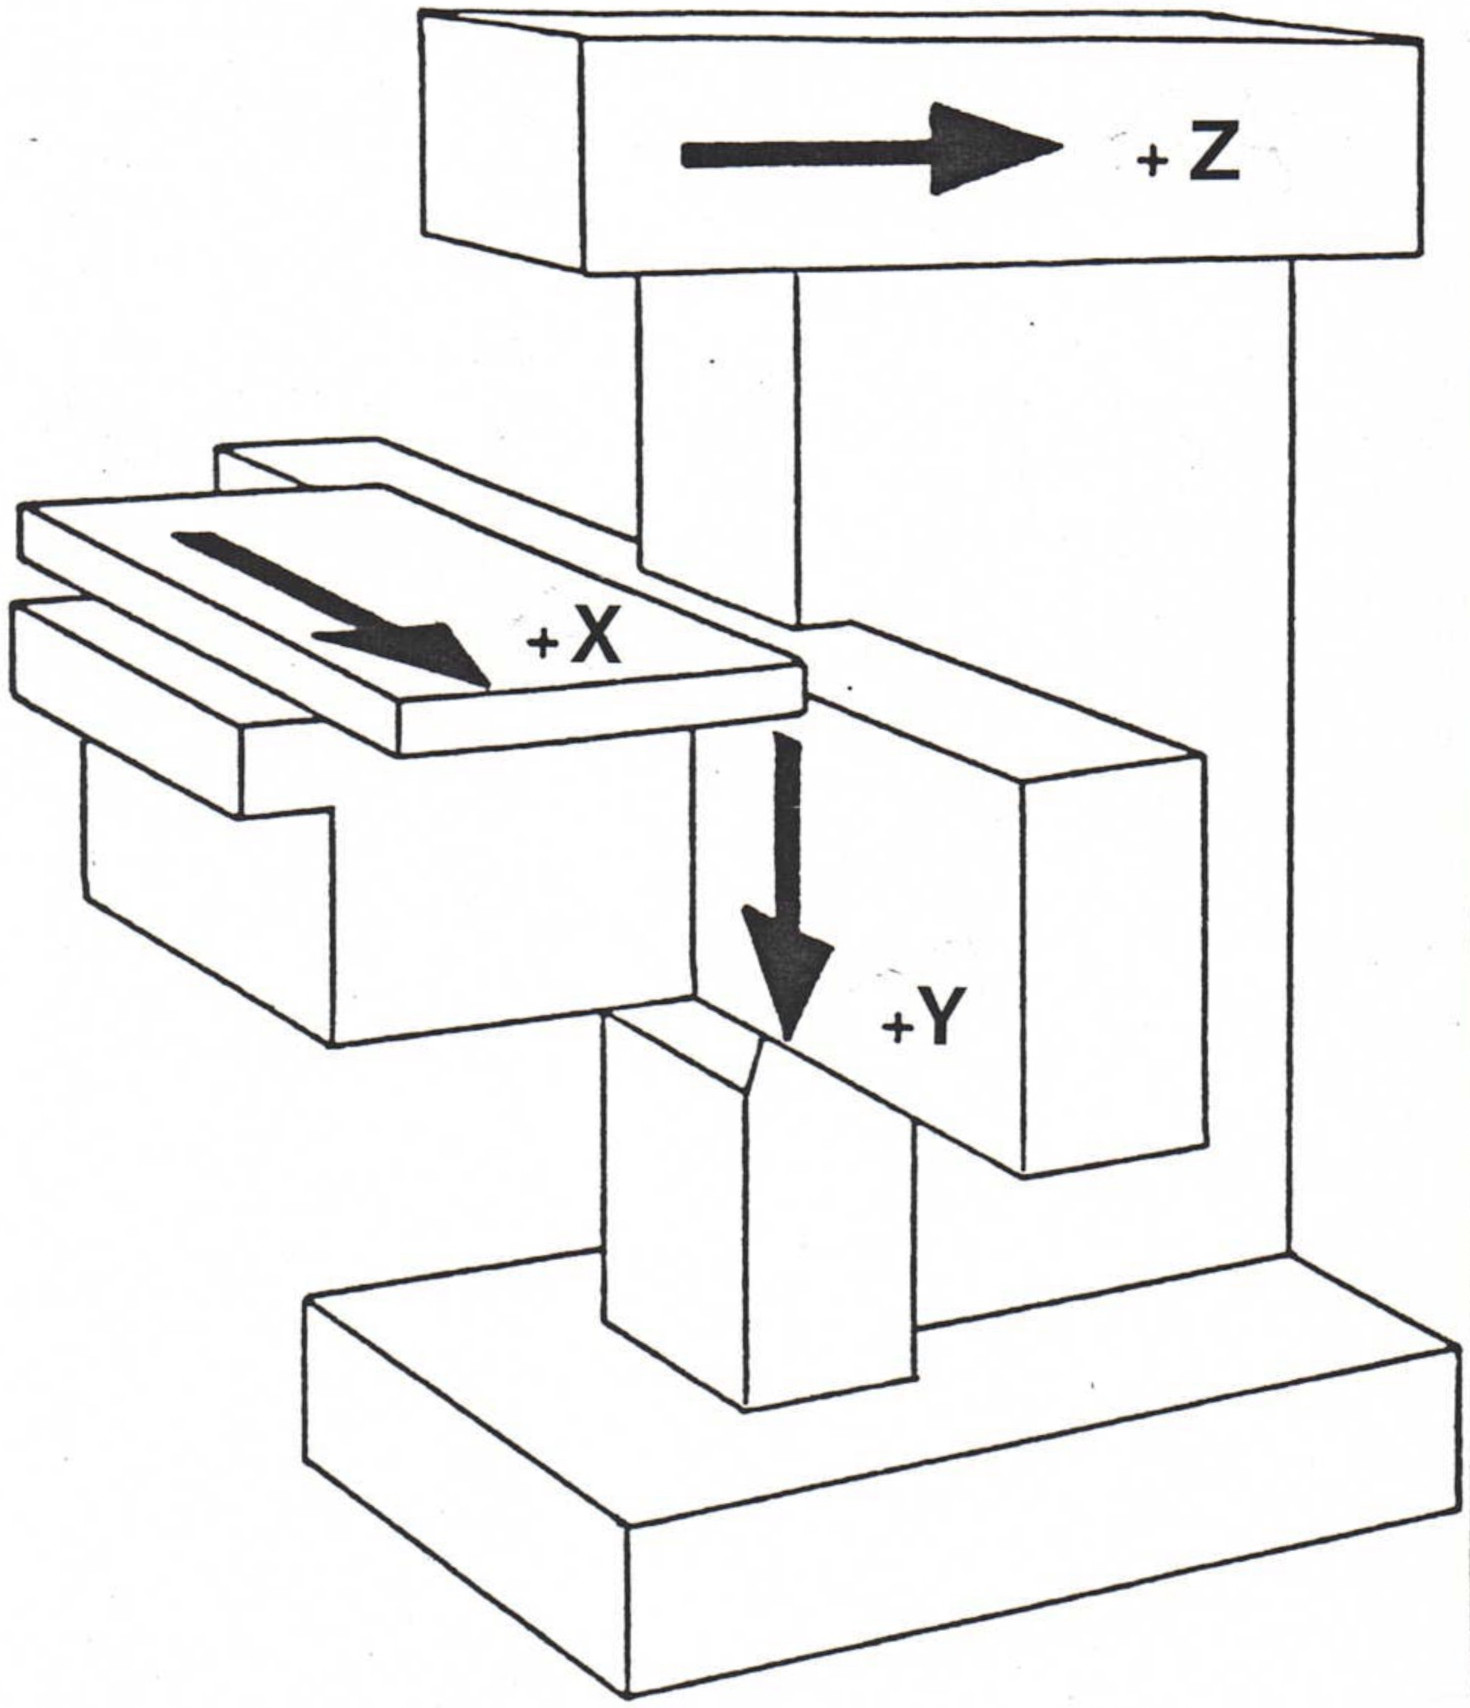
\includegraphics[width=0.8\textwidth]{chapter2/movement_directions.jpg}
\end{figure}

\vspace{0.5cm}

\textbf{Axis Definitions:}

\begin{tabular}{ l l }
\textbf{X-Axis} & Horizontal longitudinal movement of the vertical mounting table: \\
                & Left \enquote{-} or Right \enquote{+}. \\
\textbf{Y-Axis} & Vertical movement of the cross support: \\
                & Up \enquote{-} or Down \enquote{+}. \\
\textbf{Z-Axis} & Horizontal transverse movement of the spindle head: \\
                & Forward \enquote{-} or Backward \enquote{+}. \\
\end{tabular}

\setsectiontitle{Control Station (Machine)}
\setrevision{10514}

\begin{figure}[h]
    \centering
    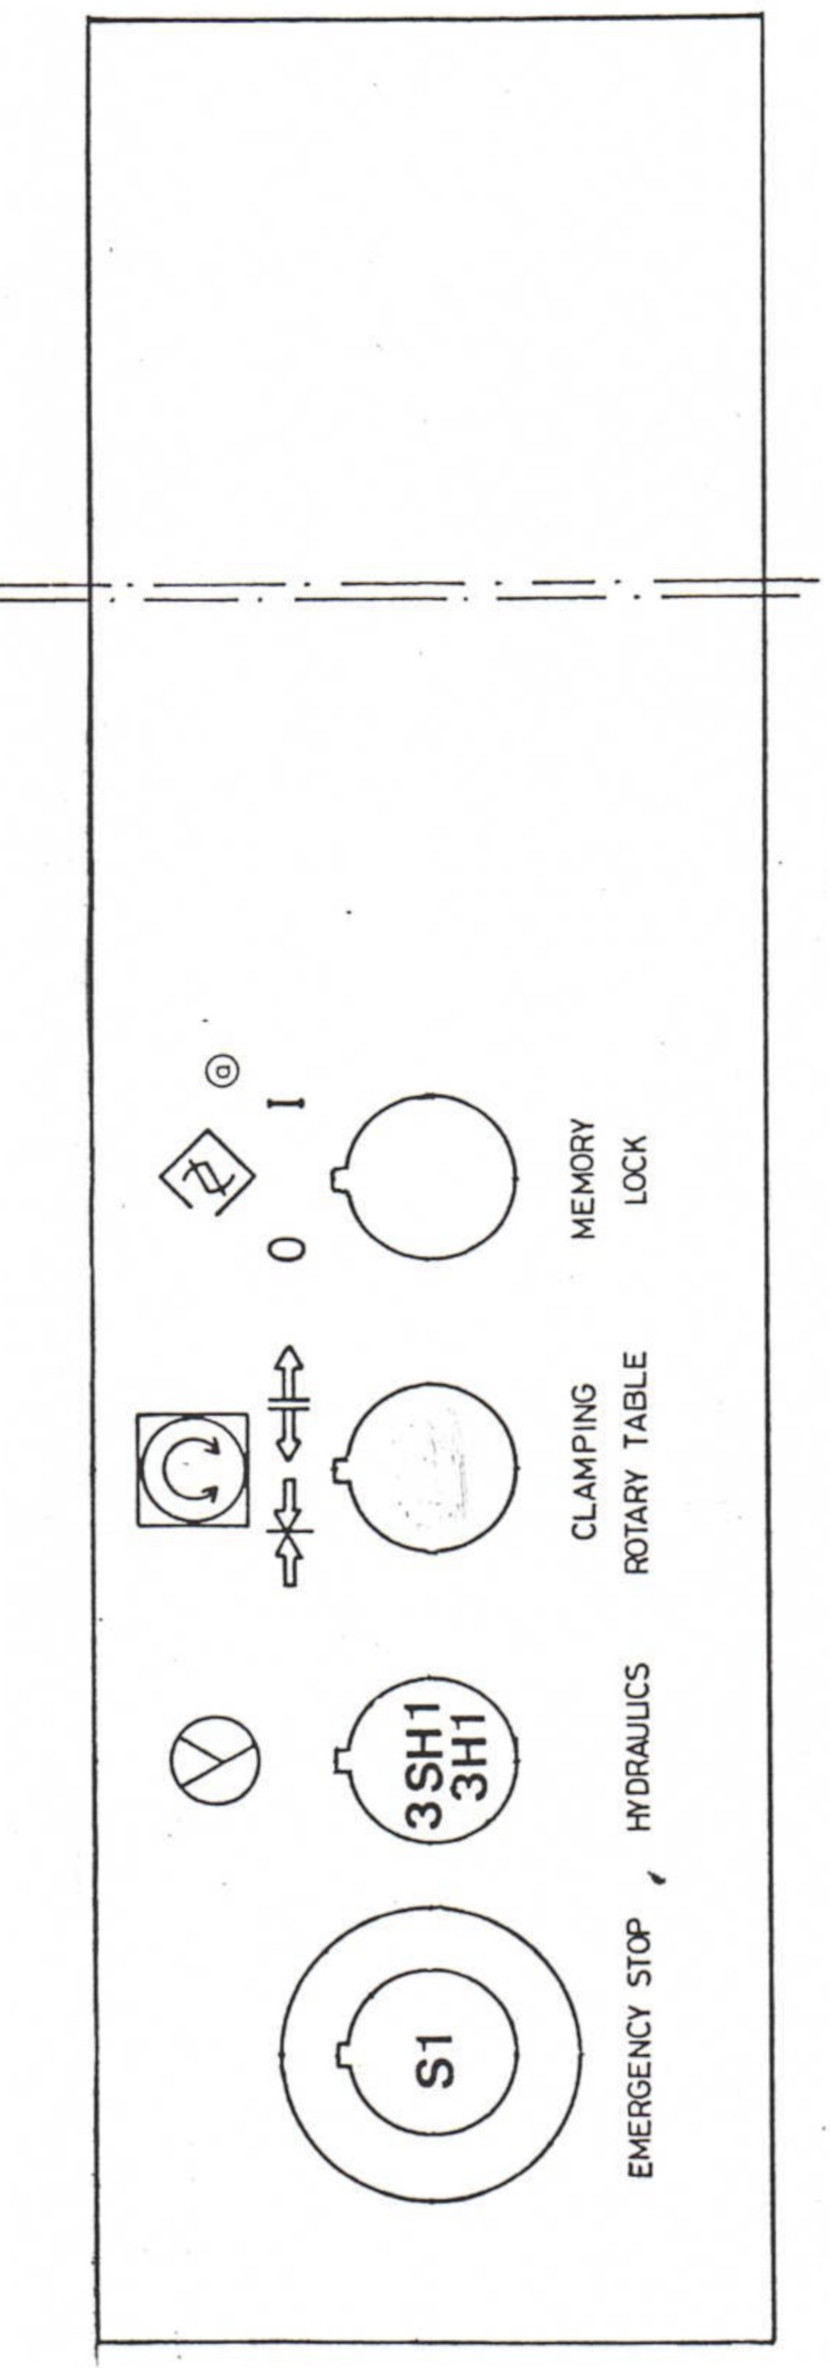
\includegraphics[width=0.38\textwidth]{chapter2/control_station.jpg} % Replace with actual filename
\end{figure}

\newpage

\subsection{Function of the Operating Elements}

\begin{tabular}{|c|l|p{10cm}|}
    \hline\hline
    \textbf{Nr.} & \textbf{Operating Element} & \textbf{Function} \\
    \hline\hline
    -S1-   & Emergency stop button & Emergency stop. All machine motors are immediately shut down.\footnotemark[11] \\
    \hline
    -3SH1- & Illuminated push button & Hydraulics, central lubrication, and control ON. \\
    -3H1-  & Indicator light & ON. \\
    \hline\hline
\end{tabular}

\vspace{0.5cm}

\footnotetext[11]{After activation, the red emergency stop button remains locked. Before restarting the machine, the locking mechanism must be released by turning the emergency stop button to the right.}

\newpage

\setcounter{page}{5}

\subsection{Handheld Control Unit}
\setrevision{5628}

For ease of setup when machining a workpiece, the CNC 432 control system is also equipped with a handheld control unit. It enables the operation of the following functions:

\begin{itemize}[itemsep=1pt,parsep=0pt]
    \item Axis selection in positive or negative direction for each axis. Operating modes: SINGLE, AUTOMATIC, MANUAL
    \item Program creation via PLAY-BACK
    \item Machine status
    \item Feed rate control (potentiometer)
    \item Spindle feed HOLD
    \item Feed START
    \item Coolant ON/OFF
    \item Tool clamp RELEASE/CLAMP
    \item EMERGENCY STOP
\end{itemize}

Safety activation is required for enabling the keyboard from the handheld control unit for safety reasons.

\vspace{0.3cm}

\notebox{NOTE}{For operation with the handheld control unit, see the separate CNC 432/Graphics operating manual.}

\vspace{0.3cm}

\notebox{WARNING}{On \enquote{E}-machines, the following keys are \uline{not activated}:}

\vspace{-0.6cm}

\begin{center}
    \fbox{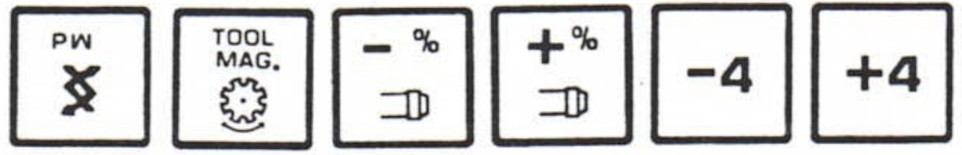
\includegraphics[width=0.4\textwidth]{chapter2/deactivated_keys.jpg}}
\end{center}

\vspace{-0.5cm}

\begin{figure}[h]
    \centering
    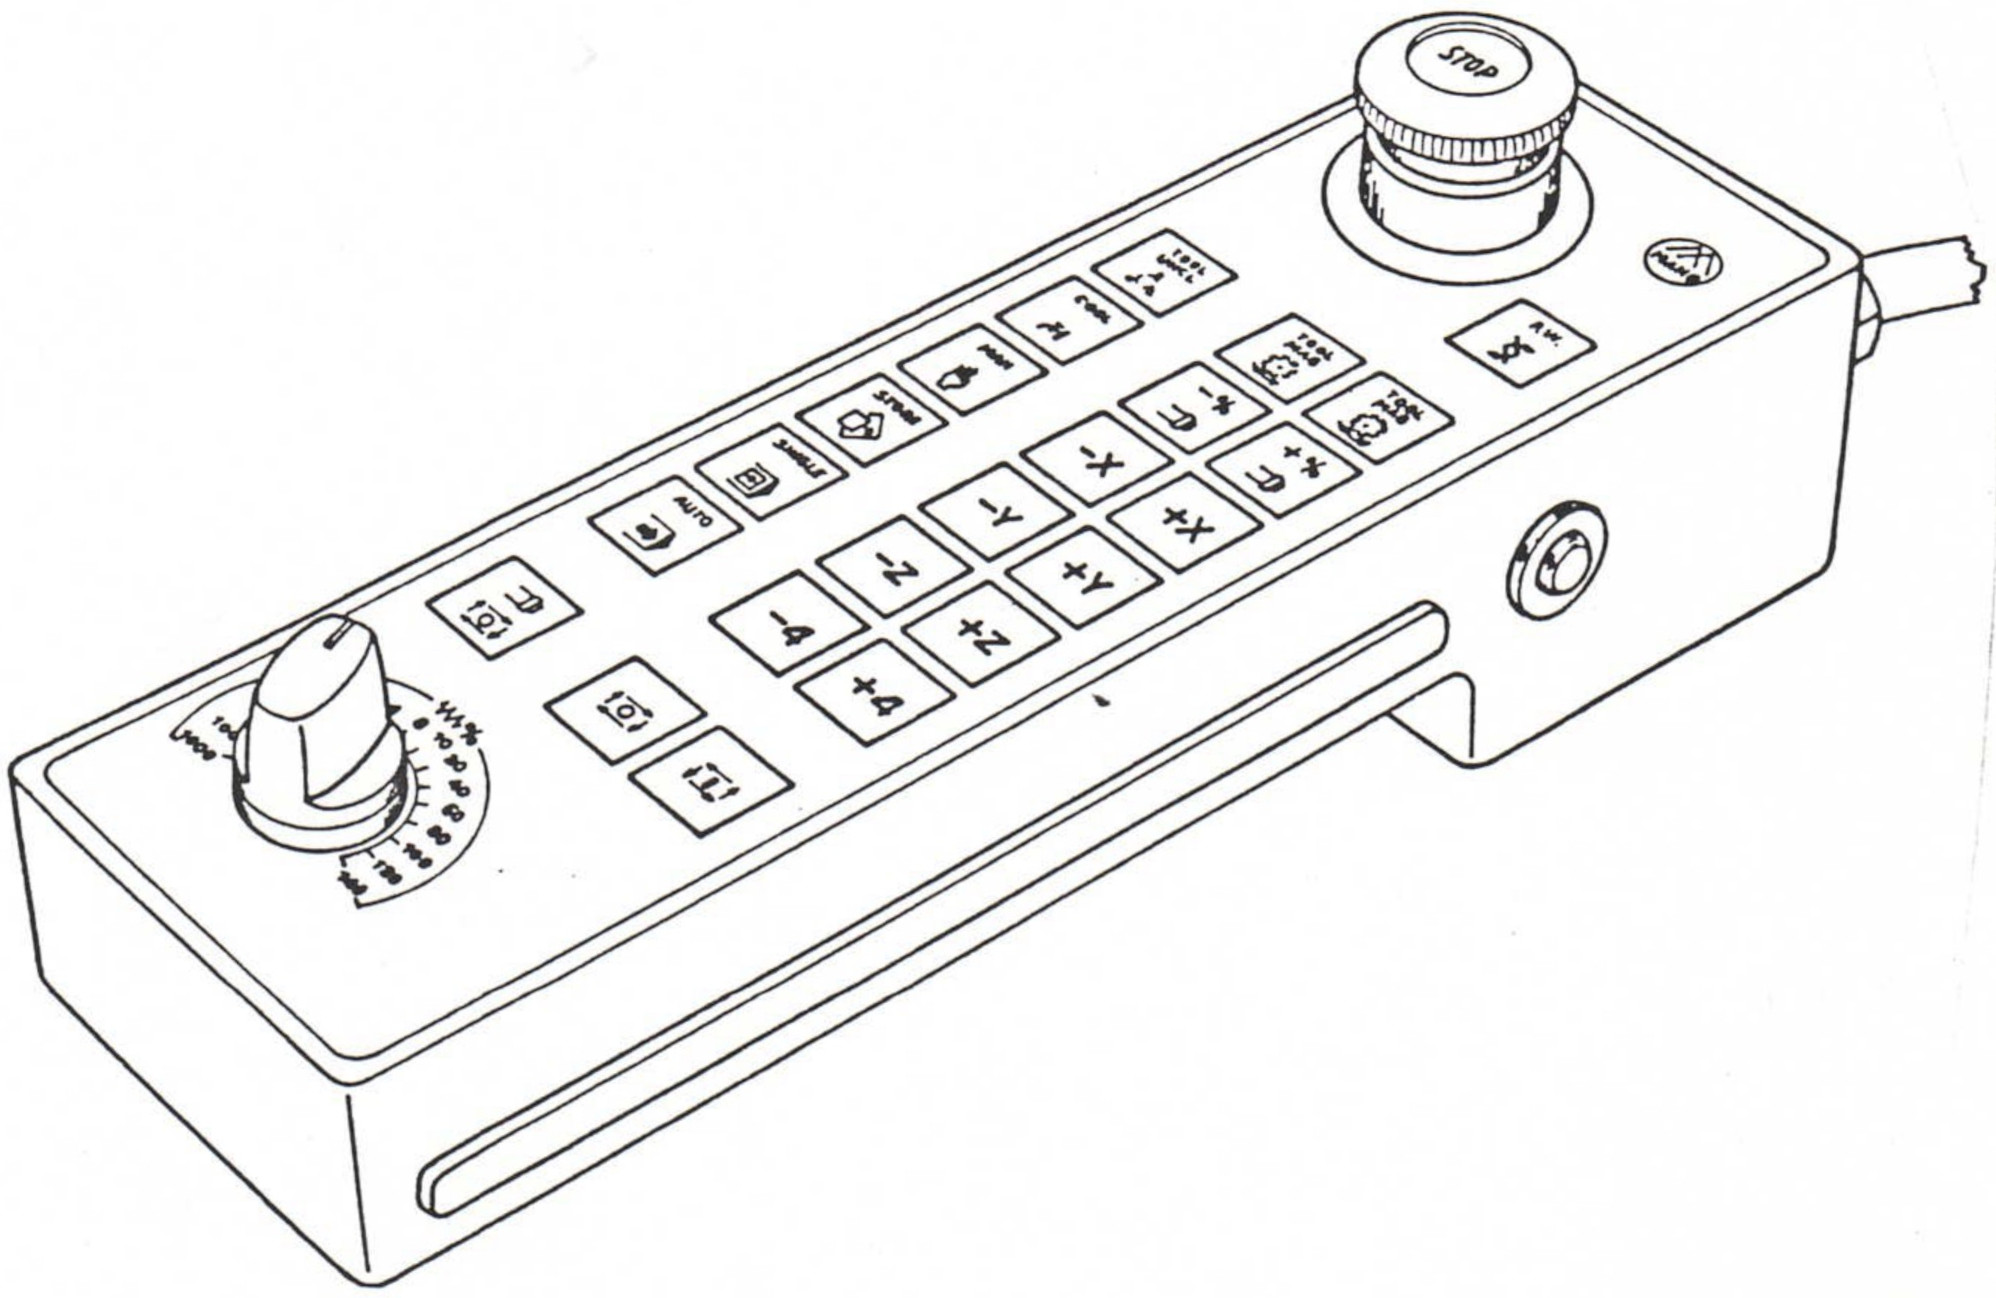
\includegraphics[width=0.9\textwidth]{chapter2/handheld_control.jpg}
\end{figure}

\setsectiontitle{Gear Train Schematic}
\setcounter{section}{10}
\begin{minipage}{\textwidth}
    \begin{adjustwidth}{-2cm}{-3cm}
        \centering
        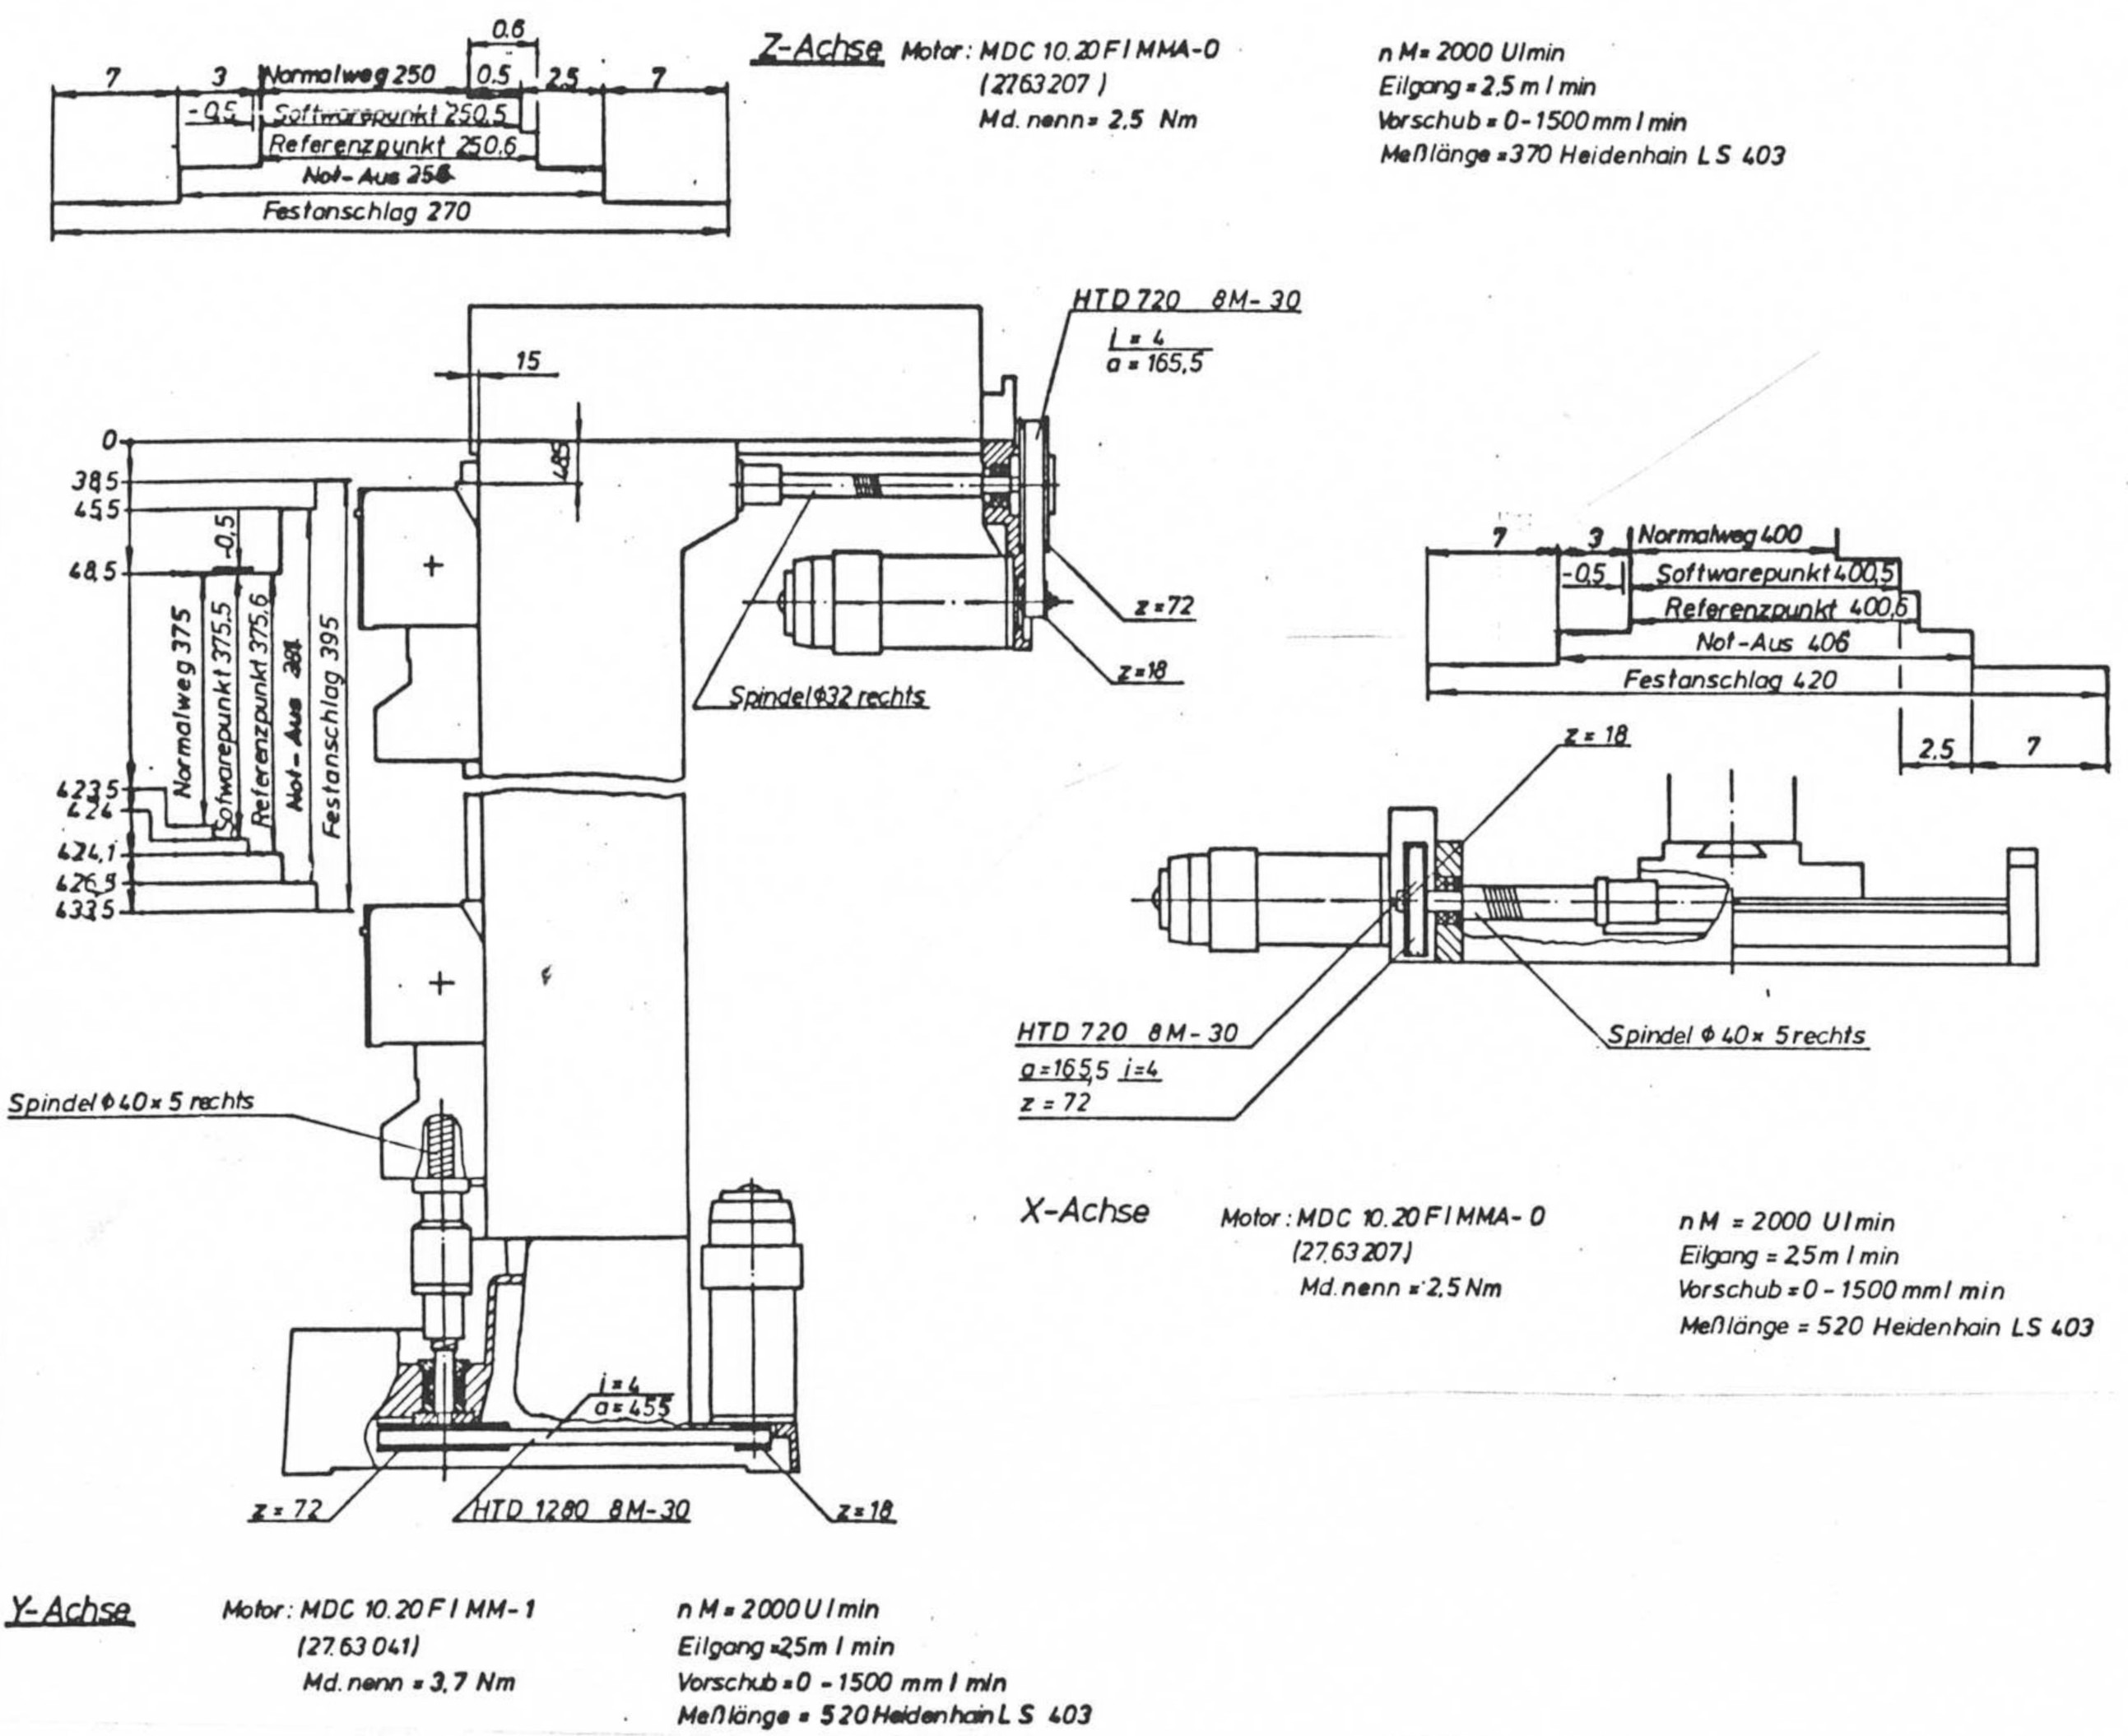
\includegraphics[angle=90,height=.9\textheight]{chapter2/gear_train_schematic.jpg}
    \end{adjustwidth}
    \label{fig:gear_train}
\end{minipage}

\newpage
\subsection[\texorpdfstring{14.48805/14.488111 (50/60Hz)}{14.48805-14.488111}]%
{Main Gearbox}
\setrevision{859}

\vspace{-.5cm}

\begin{figure}[h]
    \centering
    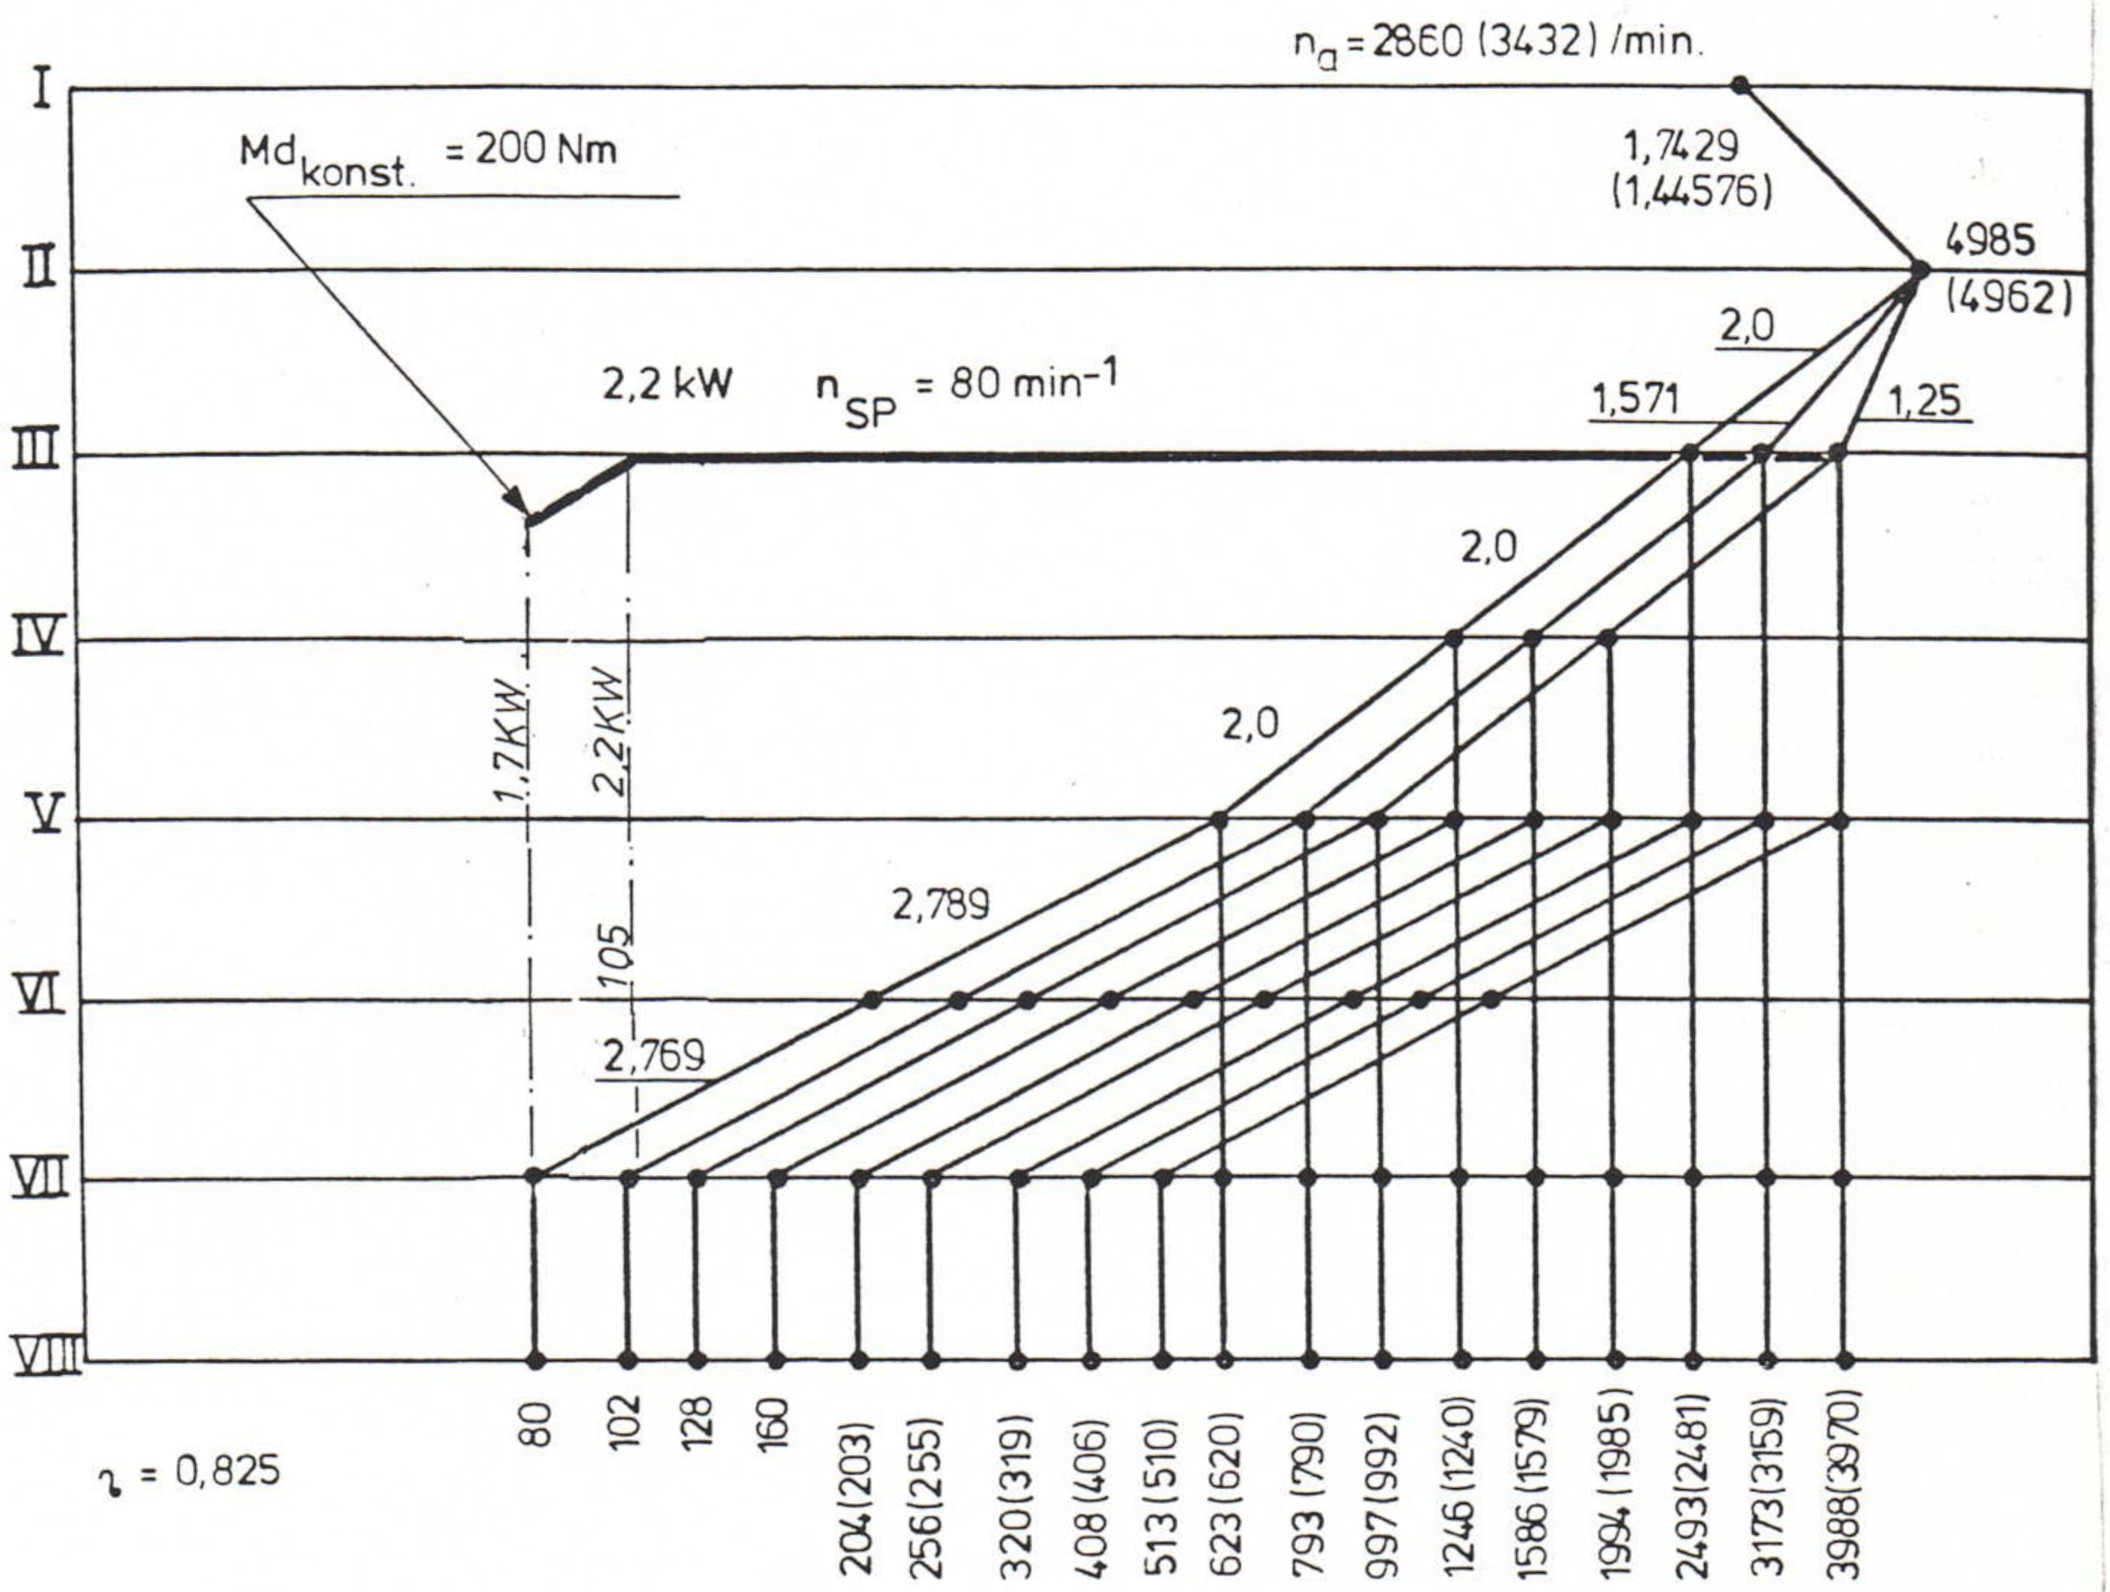
\includegraphics[width=1.05\textwidth]{chapter2/gear_train_speeds.jpg}
\end{figure}

\rule{1.08\textwidth}{0.5pt}
\footnotesize Standard Speeds: 80,100,125,160,200,250,315,400,500,630,800,1000,1250,1600,2000,2500,3150,4000
\rule{1.08\textwidth}{0.5pt}

\vspace{.5cm}

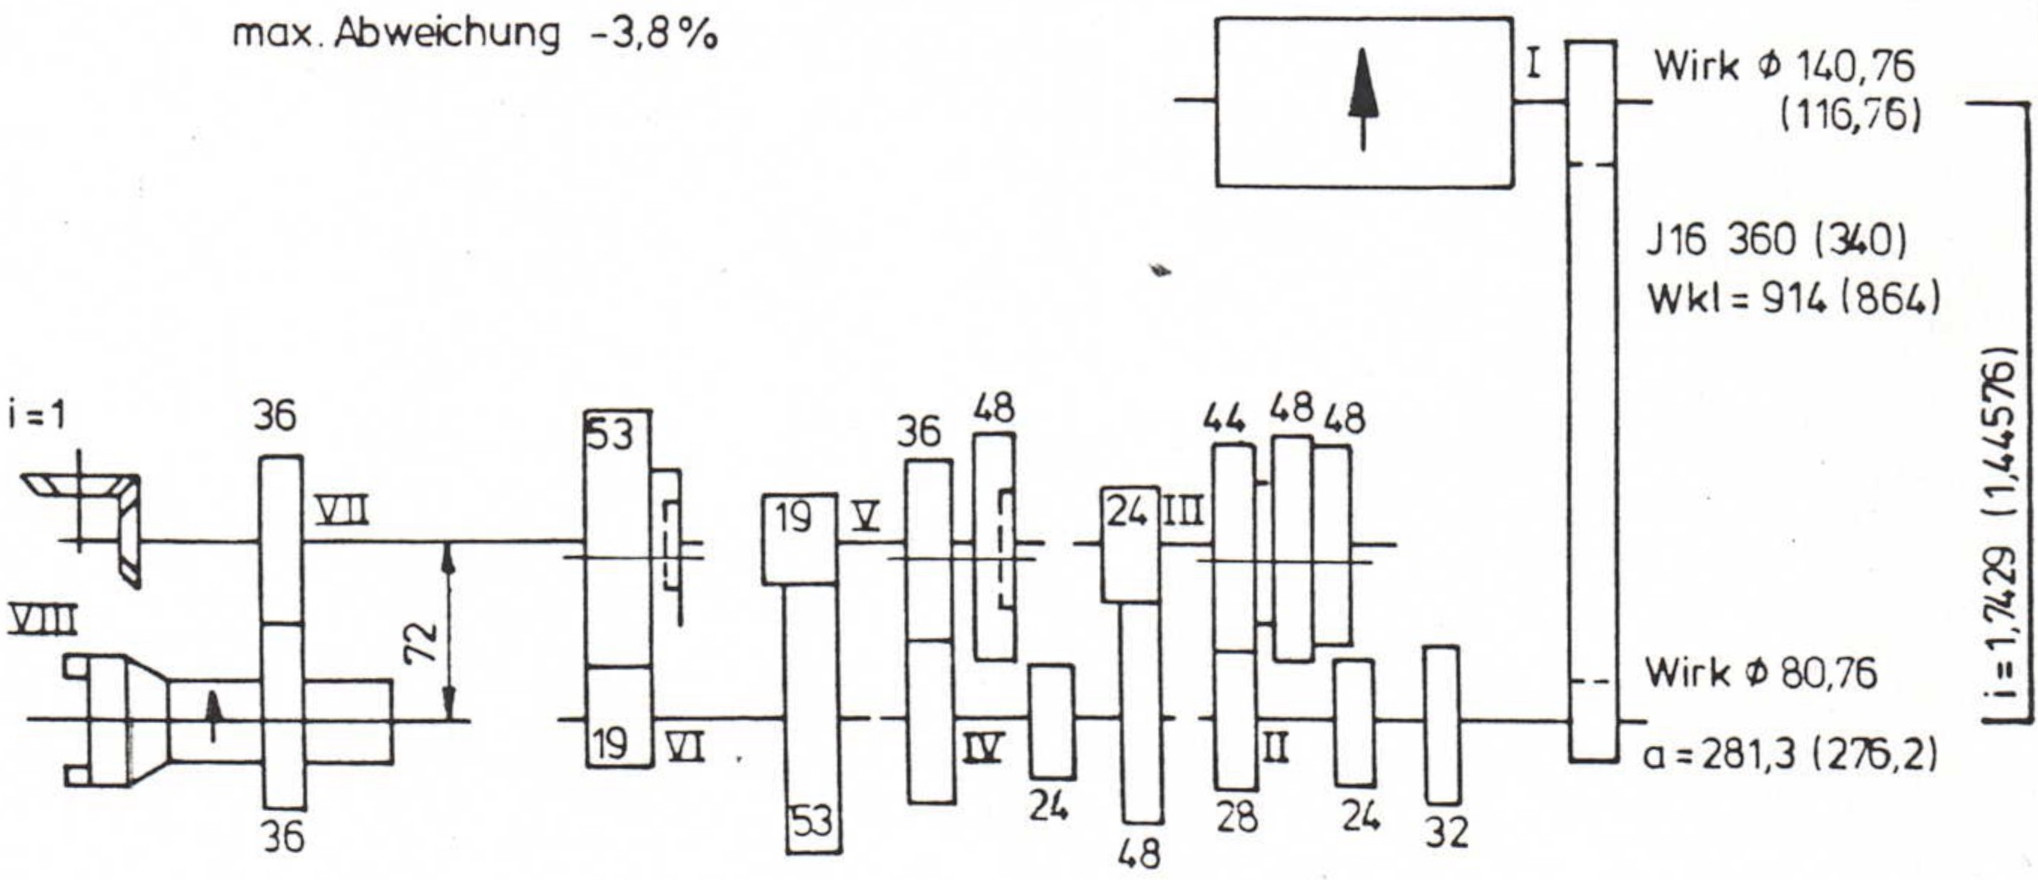
\includegraphics[width=1.02\textwidth]{chapter2/gear_train_layout.jpg}
